\section{Results}

\begin{table}
    \caption{Comparison of MAE and STDAE for original and modified pictures.}
    \label{surveytable}
\begin{tabular}{|p{0.2\linewidth}|p{0.1\linewidth}|p{0.1\linewidth}|p{0.1\linewidth}|p{0.1\linewidth}|}
    \hline
    \multicolumn{5}{|p{0.7\linewidth}|}{\centering Mean Average Error (MAE) and standard deviation of average error (STDAE) for each picture.} \\
    \hline
    \multirow{2}{0.2\linewidth}{Image name} & \multicolumn{2}{|p{0.2\linewidth}|}{Original picture} & \multicolumn{2}{|p{0.2\linewidth}|}{Our picture} \\\cline{2-5}
    & MAE & STDAE & MAE & STDAE \\
    \hline
    img0 & 6.685 & 1.039 & 5.218 & 1.166 \\
    img1 & 1.939 & 0.345 & 0.929 & 0.759 \\
    img2 & 5.491 & 0.663 & 5.397 & 0.493 \\
    img3 & 4.723 & 1.218 & 4.737 & 1.717 \\
    img4 & 5.115 & 0.858 & 3.628 & 0.723 \\
    img5 & 10.407 & 0.922 & 10.174 & 0.985 \\
    img6 & 10.647 & 1.219 & 8.937 & 1.693 \\
    img7 & 6.163 & 0.943 & 5.457 & 0.973 \\
    img8 & 2.746 & 0.659 & 1.906 & 0.904 \\
    img9 & 3.712 & 0.651 & 3.383 & 0.555 \\
    img10 & 7.029 & 0.170 & 5.676 & 0.692 \\
    img11 & 10.983 & 0.296 & 9.500 & 0.985 \\
    img12 & 4.966 & 0.417 & 3.972 & 0.985 \\
    img13 & 7.726 & 0.813 & 6.325 & 1.586 \\
    img14 & 3.738 & 0.603 & 3.000 & 1.008 \\
    \hline
\end{tabular}
\end{table}

\begin{figure}
    \centering
    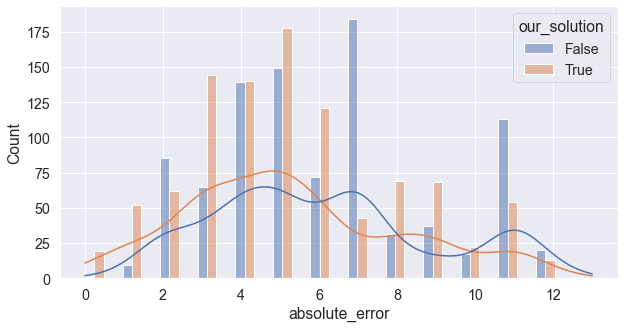
\includegraphics[width=\linewidth]{figures/survey_combined.png}
    \caption{Combined histogram of mean absolute errors of objects estimation.}
    \Description{Distributions of original and modified images are comparable but modified images are slightly better recognized.}
    \label{survey:combined}
\end{figure}


We asked people to estimate the number of objects on randomly chosen 15 pictures. We didn't record the exact number of users, but observations over IP addresses of review submissions show that about 30 different persons participated in our review producing 1930 estimations over 30 different pictures. In \autoref{surveytable} we collected mean average error and standard deviation of error of users' estimations. For all pictures except img3, we noticed that error of predictions lowered, and users started to notice more objects on the picture. However, despite the stable decline, results don't change much in absolute values. We connect this with the dataset being rather clean in terms of additional objects and different backgrounds. Since the used dataset provides a simple background (as table, floor, or carpet), reviewers are not distracted by additional obstacles that would be less noticeable on processed images. Besides that, we think that due to surveyors being unaware of key changes in the picture and not being trained, collected results could be worse than for those who understand how highlighting would emphasize the objects.

On \autoref{survey:combined} you can see the histogram of absolute errors combined for all pictures. This histogram also shows a slight improvement in recognizing the objects on the pictures, with a mean absolute error being shifted to zero compared with original images. The more detailed histograms of each picture are available in \autoref{survey:separate} in papers appendices. We noticed that the histograms support our conclusions about the changes and show stable improvement for every image except img3. 

The worse performance on img3 is closely connected with the used segmentation model. After investigating the reasons, we noticed that the segmentation model constantly highlights straight parallel lines as a possible book that leads to invalid estimations. We suggest that adjusting the model and its settings would provide better results due to the reduced number of false-positive segmented objects. In addition, we intentionally didn't finetune the model to the dataset in order to measure the performance in the wild, but in real life, such finetuning could be introduced for certain backgrounds, classes, or depending on person perception.